% !TeX root = ../../../thesis.tex

\section{AC Environment}
\label{sec:ac-environment}




The translation from an ID, that is assigned to a light fixture, to a unique current signature is more difficult in an AC environment compared to the DC environment.
This is due to the supplied voltage.
In a DC environment, the voltage is a constant value, but in an AC environment the supplied voltage is a sinusoidal wave.
This means that the voltage will be both positive and negative.
In the Netherlands the AC has an RMS voltage of 230 V and a frequency of 50 Hz.

In the next subsections, we will first describe existing hardware and their limitations.
Then new hardware is proposed to solve the limitations of the existing hardware.
Finally, the AC testbed is showcased.




% !TeX root = ../../../../thesis.tex


\subsection{Modulator}	
\label{subsec:ac-modulator}

The job of the modulator in an AC environment, is the same as in a DC environment.
Just like in the DC environment, when a `0' has to be encoded the current should be zero and when a `1' has to be encoded the current should be some constant value.
The transition between a `0' and `1' should be fast, so that a square wave is created, just like in the DC case.

If the translation is done in this manner, the mapping between the code sequence symbols and the current is clear and the aggregated current drawn by multiple lights will also be a square wave, which will allow for decoding the information.
Next, existing hardware is investigated if these solutions will translate the IDs into a current draw which is similar to what has just been discussed above. 



% !TeX root = ../../../../../thesis.tex


\subsubsection{SMPS and LED}

In \autoref{fig:ac-smps-led-and-smps-picture} a commercial LED lighting fixture can be seen with a switching mode power supply (SMPS).
The power supply transforms the AC to a DC signal which is used to power the LED.




For this setup it is investigated what the current signature looks like when the LED is on, representing a `1', and when the LED is off,  representing a `0'.
A 10 ohm resistor is placed in series with the SMPS on the AC side and the voltage drop over this resistor is measured.
So a voltage is measured, but the current that flows can be calculated using Ohm's law: $I = \frac{U}{R}$.
But since we are investigating how the current signature behaves, it is not needed to have exact numbers on the current draw.








\begin{figure}[h]
	\centering     %%% not \center
	\subfigure[Encoding a `0', LED off.]{
		\label{fig:smps-current-primary-no-load}
		\includegraphics[width=60mm]
		{chapters/hardware-chapters/AC/ac-modulator/smps-led/smps-current-primary-no-load-cropped-edit.jpg}
	}
	\subfigure[Encoding a `1', LED on.]{ 
		% 33 ohm...
		\label{fig:smps-current-primary-with-load}
		\includegraphics[width=60mm]
		{chapters/hardware-chapters/AC/ac-modulator/smps-led/smps-current-primary-with-load-cropped-edit.jpg}
	}

	\caption{Voltage measured over a 10 ohm series resistor at the primary side, to determine the current flow in two situations of a SMPS, when encoding a `0' and a `1'. X-axis: 2 ms/div, Y-axis: 500 mV/div.}
\end{figure}






In Figures \ref{fig:smps-current-primary-no-load} and \ref{fig:smps-current-primary-with-load} the current signature of the SMPS can be seen, when encoding a `0' (LED off) and when encoding a `1' (LED on), respectively.
From these figures, it is clear to see that when encoding a zero, the current is not zero and when encoding a `1', the current is not a constant value.
This makes it difficult to determine what the ID is of this transmitting LED.
This becomes even more difficult when multiple of these current signatures will be superimposed.








	\begin{figure}
		\centering
		\begin{minipage}[b]{0.45\textwidth}
			\includegraphics[width=\textwidth]{chapters/hardware-chapters/AC/ac-modulator/smps-led/smps-led-and-smps-picture.jpg}
			\caption{Picture of a commercial LED light fixture with a DC SMPS.}
			\label{fig:ac-smps-led-and-smps-picture}
		\end{minipage}
		\hfill
		\begin{minipage}[b]{0.45\textwidth}
			\centering
			\includegraphics[angle=0,width=0.5\textwidth]{chapters/hardware-chapters/AC/ac-modulator/commercial-230v-ac-led/commercial-ac-led-picture.jpg}
			\caption{Picture of a commercial 230 V AC LED light fixture.}
			\label{fig:ac-commercial-230v-ac-led}
		\end{minipage}
	\end{figure}




% !TeX root = ../../../../../thesis.tex

%\subsubsection{230 V AC LED}
\subsubsection{LEDs powered directly by 230 V AC}


There also exists LED lighting fixtures which work directly with AC, without having an external SMPS.
An example of such an LED can be seen in \autoref{fig:ac-commercial-230v-ac-led} \cite{commercial-230v-ac-led-aliexpress}.



For this LED it is investigated what the current signature looks like when the LED is constantly on, and when the LED is encoding information.
To measure the current, a 22 ohm resistor is placed in series with the light and the voltage drop over this resistor is measured.
Again, we are only looking at how the current signature behaves, at this point we are not interested in how much current is exactly being drawn.
In order to modulate the LED so that information is encoded in the current, changes had to be made to the internal hardware of the light fixture.
In \autoref{app:commercial-230v-ac-modified-schematic} a schematic can be found, which shows the original circuit and what was modified in order to modulate the LED.
The modifications made, include two transistors to switch the LEDs off and stop the capacitor from charging. 
With these transistors the entire current flow can be stopped thereby drawing zero current when we want to modulate a `0' symbol.
When a `1' symbol needs to be modulated, the transistors are turned on, and the LED behaves in a normal manner.
The transistors are controlled via a micro-controller through an optocoupler to protect the micro-controller in the development stages.



\begin{figure}[t]
	\centering     %%% not \center
	\subfigure[LED is constantly on. X-axis: 5 ms/div, Y-axis: 1 V/div.]{
		\label{fig:commercial-230v-ac-led-on-annotated}
		\includegraphics[angle=0,width=0.3\textwidth,keepaspectratio]
		{chapters/hardware-chapters/AC/ac-modulator/commercial-230v-ac-led/commercial-230v-ac-led-on-annotated.png}
	}
	\subfigure[LED is being modulated at 4 kHz. X-axis: 1 ms/div, Y-axis: 5 V/div.]{
		\label{fig:commercial-230v-ac-led-modulating}
		\includegraphics[angle=0,width=0.5\textwidth,keepaspectratio]
		{chapters/hardware-chapters/AC/ac-modulator/commercial-230v-ac-led/commercial-230v-ac-led-modulating-annotated.png}
	}

	\caption{Voltage measured over a 22 ohm series resistor at the primary side, to determine the current signature of a commercial 230 V AC LED.}
\end{figure}



When the LED is off, there is no current draw.
In Figure \ref{fig:commercial-230v-ac-led-on-annotated} the current signature can be seen when the LED is constantly on.
This figure shows 20 ms of the current signal, this is exactly one period of the supplied AC voltage: $t = \frac{1}{f} = \frac{1}{50} = 0.020$ s $= 20$ ms.
Every 20 ms this current draw repeats itself.
In the figure, three regions can be seen: A, B and C.
Each region will now be explained:

\begin{itemize}
	\item In region A, the supplied AC voltage is positive, and so the current that flows is positive.
	As can be seen from the schematic in \autoref{app:commercial-230v-ac-modified-schematic}, all the LEDs are connected in series.
	This means that a certain voltage is required in order for the LEDs to draw current.
	The required voltage is available at the start of region A and is no longer available at the end of region A and the current flow stops.
	The width of the peak is 4 ms.
	This is because in those 4 ms, there is enough voltage available to power all the LEDs in series. 
	The height of the peak indicates how much current is drawn.

	\item The start of region B starts when region A stops.
	The required voltage is no longer available and so the current flow stops and the LED no longer emits light.
	During this region there is no current flow.
	This is a good property: If the LED is off there is no current flow, exactly what we require.

	\item Region C starts when region B stops.
	At this point in time, there is enough voltage available for the LEDs to start drawing current again.
	But the voltage that is now available, is not positive as it was in region A, but is negative.
	That is why this peak goes the opposite direction of the peak seen in region A.
	The current that flows is in that case negative, because the voltage is also negative.
	In other aspects this peak has the same properties as those of the peak in region A, it has the same width and height.

\end{itemize}


Only in region A and C, the LED can be used to encode information.
Because in region B, the is no current draw and therefor we cannot modulate information.
The peaks in region A and C are both 4 ms wide.
This means that there is 8 ms of time available for modulation in the 20 ms period, so $\frac{8}{20} = 40$ \% of the time is available for encoding the ID with this LED.
To compare with a DC environment: In a DC scenario, the power supply always supplies a constant voltage, so the LED can always emit light and therefor can always draw current, so 100 \% of the time is available for modulation.
If the ID would have a certain length, it would take time $t$ to modulate this ID in a DC environment and time $2.5 \times t$ with this AC LED if the ID could not be transmitted inside the 4 ms window. 


Now that the current signature has been investigated when the LED is on, the LED will be now be turned on and off with a frequency of 4 kHz to investigate how the current signature behaves.
In Figure \ref{fig:commercial-230v-ac-led-modulating} the current signature can be seen when the LED is being modulated with a frequency of 4 kHz.
The entire figure takes place inside region A of Figure \ref{fig:commercial-230v-ac-led-on-annotated}.
If this figure would have been showed for region C of Figure \ref{fig:commercial-230v-ac-led-on-annotated}, the amplitudes would have been negative.
Again, there are three regions highlighted:

\begin{itemize}

	\item In region A, the data being encoded is a `0' and the current draw is also zero.
	As discussed this is a desired property.

	\item Region B shows the transition from the LED being off to the LED being on.
	The current does not go straight up, but instead a slope can be seen.
	This is not a desired property.
	A square wave is desired, this LED is producing a triangular wave.

	\item In region C, the transition from the LED being on to the LED being off can be seen.
	This time the current does go immediately to zero, which is a good property.
	Around region C another issue can be seen. 
	The amplitude of the current becomes lower and lower until region A of Figure \ref{fig:commercial-230v-ac-led-on-annotated} ends.
	This is also not a desirable property, the current should always be some constant value and not decreasing over time.

\end{itemize} 



From this investigation it can be concluded that this 230 V AC LED is not suitable to map the ID into the current signature which is desired.
And also the time that would be available for modulation is limited, because there are many LEDs in series which require a high voltage which is only available for a short amount of time.











% !TeX root = ../../../../../thesis.tex

\subsubsection{Custom AC Modulator}






Given the shortcomings of the existing hardware, it was decided to build custom hardware that would behave exactly how it was needed in order to successfully encode information in such a way that the currents could be decoded by a smart-meter.
This means that the current signature should behave very similar to the DC case: For a `0' data bit encoding, the current should be zero and for a `1' data bit encoding, the current should be some constant value.
The transitions between the symbols must be such, that a square wave of current will be created, just like in the DC case. 

\begin{figure}[h]
	\centering
	\includegraphics[angle=0,width=0.7\textwidth]{chapters/hardware-chapters/AC/ac-modulator/custom-hardware/ac-modulator-architectural.JPG}
	\caption{Architectural overview of the AC LED modulator.}
	\label{fig:ac-led-modulator-architectural}
\end{figure}

The custom modulator consists of three separate parts: A trigger circuit, a current source and a voltage source.
In \autoref{fig:ac-led-modulator-architectural}, an overview of how these parts are connected to each other can be seen.
The commercial LED that will be used for this solution was already shown \autoref{fig:ac-smps-led-and-smps-picture}, but the SMPS is not used, instead this custom hardware will be powering the LED. 
The entire modulator's schematic can be found in \autoref{app:custom-led-modulator-schematic}.
In the following subsections each part of the hardware of the custom LED modulator will be explained.



	\subparagraph{Triggering}
	\label{subsubsec:triggering}

	As discussed in \autoref{subsubsec:ac-230v-led}, LEDs need a certain amount of voltage before they draw current.
	That is why Figure \ref{fig:commercial-230v-ac-led-on-annotated} has two separate regions where it draws current, instead of drawing current continuously.
	Given the fact that the ID of the LED cannot be transmitted the entire time, due to voltage issue, we must somehow give the micro-controller a signal for when the modulation can start and stop.
	If the micro-controller does not have this information, bits of the ID would be encoded when there is not current draw and thus information would be lost.

	To let the micro-controller know when to start and stop modulating, a triggering circuit is designed.
	This circuit tells the micro-controller when more than a preset voltage is made available by the AC power.
	It also tells the micro-controller when there is less than the preset voltage available.
	In \autoref{fig:triggering-circuit-output-2} the AC voltage can be seen, along with the preset voltage and the corresponding logical output of the triggering circuit.

	%\begin{figure}[h]
	%	\centering
	%	\begin{minipage}[b]{0.39\textwidth}
	%		\includegraphics[width=\textwidth]{chapters/hardware-chapters/AC/ac-modulator/custom-hardware/triggering-circuit-output-cropped.png}
	%		\caption{Output from the triggering circuit. Settings: 2 V/div, 2 ms/div.}
	%		\label{fig:triggering-circuit-output}
	%	\end{minipage}
	%	\hfill
	%	\begin{minipage}[b]{0.49\textwidth}
	%		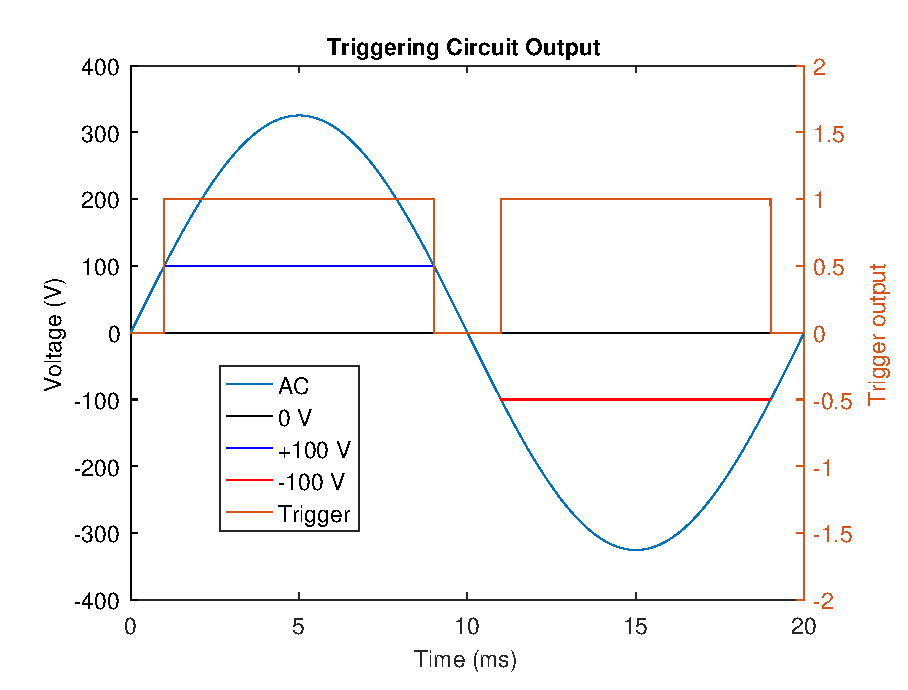
\includegraphics[width=\textwidth]{chapters/hardware-chapters/AC/ac-modulator/custom-hardware/ac-wave-triggering.eps}
	%		\caption{Output form the triggering circuit alongside the incoming AC voltage.}
	%		\label{fig:triggering-circuit-output-2}
	%	\end{minipage}
	%\end{figure}


	\begin{figure}[h]
		\centering
		\begin{minipage}[b]{0.49\textwidth}
			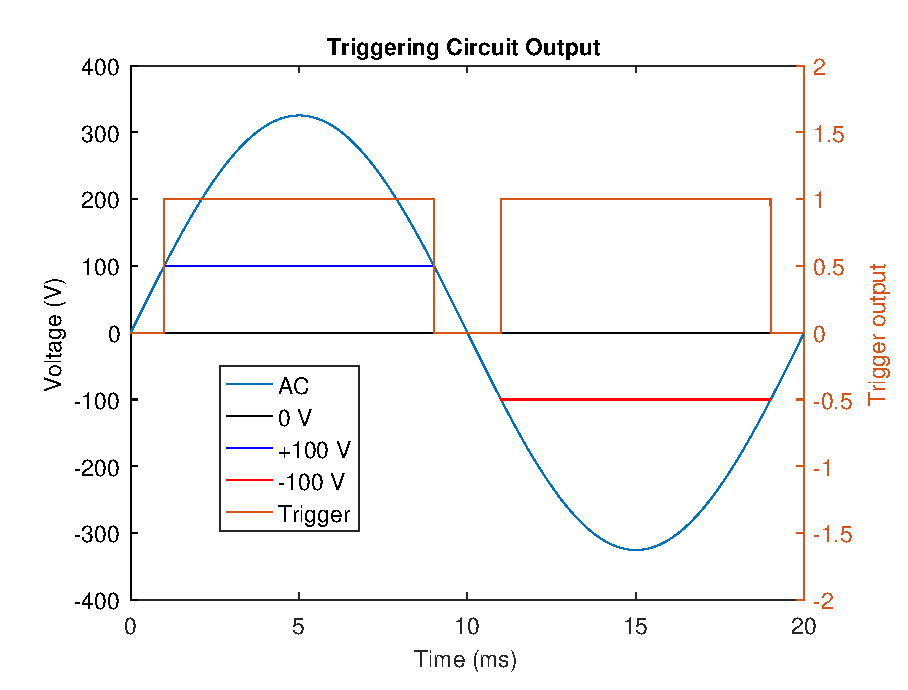
\includegraphics[width=\textwidth]{chapters/hardware-chapters/AC/ac-modulator/custom-hardware/ac-wave-triggering.eps}
			\caption{Output form the triggering circuit alongside the incoming AC voltage.}
			\label{fig:triggering-circuit-output-2}
		\end{minipage}
		\hfill
		\begin{minipage}[b]{0.49\textwidth}
			\includegraphics[width=\textwidth]{chapters/hardware-chapters/AC/ac-modulator/custom-hardware/custom-modulator-trigger.JPG}
		    \caption{Triggering circuit to determine when the voltage is sufficiently high enough to start encoding the ID.}
			\label{fig:custom-modulator-trigger}
		\end{minipage}
	\end{figure}

	In \autoref{fig:triggering-circuit-output-2}, the preset voltage is set at 100 V.
	When more than 100 V is available the LED will emit light and start drawing current.
	At that point, around 1 ms in the figure, the triggering circuit will output a logical `1' to the micro-controller, meaning that the encoding of the ID may start.
	When less than 100 V is available, around 9 ms in the figure, the logical output of the circuit becomes `0', indicating to the micro-controller that it is time to stop encoding the ID, because else information is lost since the LED is not turning on anymore.
	The same happens for the negative part of the sine wave, except the preset is now $-100$ V.


	From \autoref{fig:triggering-circuit-output-2} it can be deduced that two times 8 ms is available to encode the ID in a period of 20 ms.
	So $\frac{2 \times 8}{20} = 80$ \% of the time is available for modulation, which is two times more than the solution in \autoref{subsubsec:ac-230v-led} provided.
	To transmit the ID, this solution would be two times faster, but it would still take 25 \% more time than in a DC environment.



	In \autoref{fig:custom-modulator-trigger}, the circuit can be seen which signals the micro-controller when the voltage is more or less than the preset voltage. 
	The voltage preset can be set by using a potentiometer.
	The output of the circuit is electrically isolated from the micro-controller by the means of an optocoupler.
	This is done to protect the micro-controller from the high voltage AC in the development stages.








	


	




	%Both figure side by side to save space...
	%\begin{figure}[!tbp]
	%  \centering
	%  \begin{minipage}[b]{0.48\textwidth}
	%    \includegraphics[width=\textwidth]{chapters/hardware-chapters/custom-modulator-trigger.JPG}
	%    \caption{Triggering circuit to determine when the voltage is sufficiently high enough to start encoding information.}
	%	\label{fig:custom-modulator-trigger}
	%  \end{minipage}
	%  \hfill
	%  \begin{minipage}[b]{0.48\textwidth}
	%    \includegraphics[width=\textwidth]{chapters/hardware-chapters/custom-modulator-voltage-source.JPG}
	%    \caption{Non-disturbing voltage source to power other parts of the circuit.}
	%	\label{fig:custom-modulator-voltage-source}
	%  \end{minipage}
	%\end{figure}

	\subsubsection{Non-disturbing Voltage Source}
	\label{subsubsec:non-disturbing-voltage-source}

	The triggering circuit (\autoref{fig:custom-modulator-trigger}) requires a 5 V power supply.
	This voltage must be provided by a voltage source that will not distort the current draw.
	Otherwise it might disturb how the code sequence is translated in the current draw.

	Since the triggering circuit determines when the encoding may start, the voltage source can operate before the encoding starts.
	In that way it will not distort the encoding, because no encoding takes place yet.
	The schematic found in \autoref{fig:custom-modulator-voltage-source} provides a stable 5 V output.
	By only drawing current when there is no encoding being done, the voltage that the AC is providing is low, but still above 5 V.
	The AC voltage is then being used to charge a capacitor, that goes to a voltage stabilizer.
	The capacitor can then provide enough power for the triggering circuit until the capacitor can be charged again.


	%\begin{figure}[htb]
	%	\includegraphics[angle=0,width=\textwidth]{chapters/hardware-chapters/custom-modulator-voltage-source.JPG}
	%	\caption{Non-disturbing voltage source to power other parts of the circuit.}
	%	\label{fig:custom-modulator-voltage-source}
	%\end{figure}



	\subsubsection{Current Source}
	\label{subsubsec:current-source}


	For the current to be drawn instantaneously when the microprocessor tells the LED to turn on and to always be the same amount of current, a current source is implemented. 
	This will solve the problems that the other solutions have, such as: a non-constant current draw and a non-instantaneous current draw but a slope.
	The toggling of the current source on and off must be isolated from the microprocessor, to protect the microprocessor in the development stages, for this an optocoupler is used.
	The schematic can be found in \autoref{fig:custom-modulator-current-source}.
	The current that is drawn by the current source when modulating can be seen in \autoref{fig:current-source-measurement}.
	As seen in the figure the current goes both positive and negative, because of the AC, but the current itself is always a constant value, no matter if the current source is on or off.
	The two peaks in the figure are the charging peaks for the capacitors as discussed in \autoref{subsubsec:non-disturbing-voltage-source}.


	However, this solution also has a drawback.
	The current source will make sure a constant amount of current will flow through the LEDs.
	The current that flows through the LEDs will cause a voltage difference over the LEDs.
	This is the voltage the LEDs need in order to be turned on, as discussed in \autoref{subsubsec:triggering}.
	The rest of the voltage that the AC delivers will have to go somewhere.
	This voltage will be dissipated over the current source.
	This means that some energy is now being wasted, because there is more voltage provided by the AC than is needed to power the LEDs.

	One solution for this is using a transformer.
	This will scale down the voltage, but it will still remain a sinusoidal wave.
	But the same amount of voltage is still required by the LEDs.
	And if the sine wave now has a smaller amplitude, the time that is left for modulation will also be much smaller.
	This can be seen in \autoref{fig:trigger-output-lower-transformed}.
	Here the same voltage is required by the LEDs, 100 V.
	But the incoming sine wave has a smaller amplitude because a transformer, transformed the 230 V AC to a lower voltage.
	The time that is now available for modulation is 6 ms, which means that only $\frac{6}{20} = 30$ \% of the time is now available for modulation.
	Another drawback is that the transformer will deform the distinct current pattern that we are trying to create, as no ideal transformers exist.

	Another solution was thought of and also implemented in the circuit boards but due to lack of time it was not further experimented with.
	The solution is made up out of two parts: A capacitor and a zero-crossing opto-triac.
	The capacitor is place in series with incoming AC to the rectifying bridge.
	And the opto-triac is parallel to this capacitor.
	The schematic can be seen in \autoref{fig:ac-capacitor-triac}.
	The capacitor with AC acts as a kind of resistor so it will limit the power that is dissipated by the current source, but the capacitor itself will not dissipate any power.
	However by limiting the power that the current source will dissipate the amplitude of the sine will also become smaller and then there is much less time available to modulate, similar to the solution with the transformer as described above.
	This is were the zero-crossing triac comes in.
	Whenever it is decided to start modulating, the microcontroller activates the triac and then it will short-circuit the capacitor when the voltage is zero, so that no current will flow through the triac and thereby not damaging the triac.
	Now the capacitor is bypassed and modulation can begin with a large time available for modulation.
	When the modulation is done, the triac is switched off and the capacitor limits the power once again.
	The drawback that comes with this is that the capacitor can limit the power by phase-shifting the current as seen from the voltage.
	But the current will not be phase-shifted when the triac is active.
	So this solution is a complicated one, but it can solve the problem that the current source is dissipating excessive power.
	But it also introduces a lot of complexity and there was no more time to evaluate the benefits and drawbacks of this solution.




	%\begin{figure}
	%	\centering
	%	\includegraphics[angle=0,width=0.5\textwidth]{chapters/hardware-chapters/ac-capacitor-triac.JPG}
	%	\caption{Schematic to show how the capacitor and opto-triac are connected.}
	%	\label{fig:ac-capacitor-triac}
	%\end{figure}


	%\begin{figure}[!tbp]
	%  \centering
	%  \begin{minipage}[b]{0.49\textwidth}
	%    \includegraphics[width=\textwidth]{chapters/hardware-chapters/ac-capacitor-triac.JPG}
	%	\caption{Schematic to show how the capacitor and opto-triac are connected.}
	%	\label{fig:ac-capacitor-triac}
	%  \end{minipage}
	%  \hfill
	%  \begin{minipage}[b]{0.49\textwidth}
	%    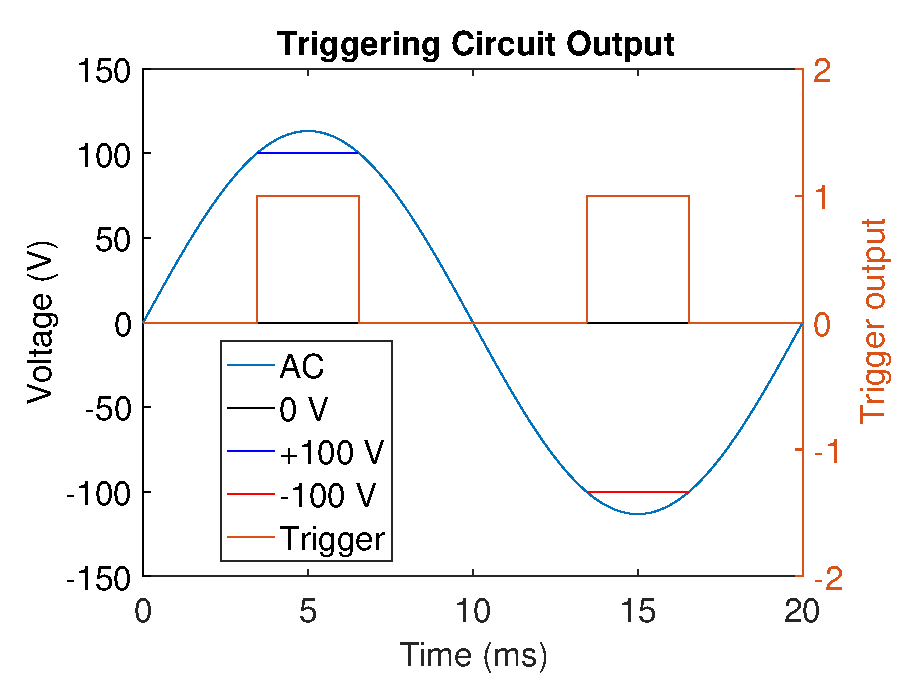
\includegraphics[width=\textwidth]{chapters/hardware-chapters/ac-wave-lower-transformed-triggering.eps}
	%    \caption{Output triggering circuit alongside the output of the AC voltage after a transformer.}
	%    \label{fig:trigger-output-lower-transformed}
	%  \end{minipage}
	%\end{figure}
%
%
%	%%\begin{figure}[htb]
%	%%	\centering
%	%%	\includegraphics[angle=0,width=0.5\textwidth,keepaspectratio]{chapters/hardware-chapters/custom-modulator-current-source.JPG}
%	%%	\caption{Current source to power the commercial LED fixture, can be toggled on and off with a microprocessor.}
%	%%	\label{fig:custom-modulator-current-source}
%	%%\end{figure}
%
%	%\begin{figure}[!tbp]
%	%  \centering
%	%  \begin{minipage}[b]{0.49\textwidth}
%	%    \includegraphics[width=\textwidth]{chapters/hardware-chapters/custom-modulator-current-source.JPG}
%	%	\caption{Current source to power the commercial LED fixture, can be toggled on and off with a microprocessor.}
%	%	\label{fig:custom-modulator-current-source}
%	%  \end{minipage}
%	%  \hfill
%	%  \begin{minipage}[b]{0.49\textwidth}
%	%    \includegraphics[width=\textwidth]{chapters/hardware-chapters/current-source-measurement-cropped.png}
%	%    \caption{Current that is drawn by the current source. Measured over an 2.8 Ohm resistor. Settings: 200 mV/div, 2 ms/div.}
%	%	\label{fig:current-source-measurement}
%	%  \end{minipage}
%	%\end{figure}
%















% !TeX root = ../../../../thesis.tex


\subsection{Current Sampler}
\label{subsec:ac-current-sampler}


Now that there exists a solution to encode the ID of an LED into the current draw, as explained in \autoref{subsec:ac-modulator}, it is now time to explore the possibilities to measure the current.
The measured current can then be processed by a micro-controller, and then the status of the LEDs can be determined.


To measure the AC current, first existing solutions were investigated.
One such a product is a `Hall Effect-Based Linear Current Sensor' \cite{hall-ac-current-sensor-datasheet}.
Based on the Hall effect, this sensor outputs a voltage which is proportional to the current that goes through the sensor.
This sensor has the issue that the noise is larger than the voltage signal which is outputted using the provided LEDs.
According to \cite{hall-ac-current-sensor-datasheet}, the highest sensitivity is $185$ mV / A and the noise is rated at $21$ mV.
The commercial LED fixtures which were provided, are rated at $15$ Watts.
With the 230 V AC, this works out to a current of $I = \frac{P}{U} = \frac{15}{230} = 0.065$ A.
At that current the output voltage will be $185 \times 0.065 = 12$ mV.
The noise of the output is $21$ mV, which is almost double the output voltage when one LED is on.
This sensor would not be able to reliably detect one or two LEDs.



Another solution has to be used to overcome the noise problem of the Hall effect sensor.
This solution has two parts: The current sampler itself and a triggering circuit.

The triggering circuit is needed to know when the modulators start and stop encoding the ID.
This will help the smart-meter, by telling it when to start and stop looking for the IDs of the LEDs.
The triggering circuit is the same circuit that was used for the modulator, which was explained in \autoref{subsec:ac-modulator}.
The part which samples the current will be explained next, but first an overview is given of how the different parts of the smart-meter are connected in \autoref{fig:ac-current-sampler-architectural}.
The meter is placed in series with an incoming AC power-line and the LEDs will be connected with the AC output.
The current-sampler forwards information about the current draw to a micro-controller for processing.
And the triggering circuit detects when the voltage is high enough for modulation for the LEDs. 


\begin{figure}[h]
	\centering
	\includegraphics[angle=0,width=0.7\textwidth,keepaspectratio]{chapters/hardware-chapters/AC/ac-current-sampler/ac-current-sampler-architectural.JPG}
	\caption{Architectural overview of the AC current sampler.}
	\label{fig:ac-current-sampler-architectural}
\end{figure}


For the current-sampler itself a resistor will be used, since this approach ensures that no noise will be introduced to the sampled current signal.
As could be seen from \autoref{fig:custom-modulator-current-source}, the current that flows is both positive and negative, due to the nature of the AC that is used.
This means that the voltage that is measured over the resistor will also be positive and negative.
An ADC (Analog-to-Digital Converter) cannot measure a negative voltage.
So the voltage over the resistor is summed with another voltage to ensure that the ADC will always measure a positive voltage.
This other voltage comes from a reference voltage IC \cite{lm336z-ref-voltage-datasheet}, which outputs a very stable reference voltage often used in scenarios where an ADC is used to measure analog signals.

At this point the ADC is measuring the voltage over a resistor which is in series with the ground (N) or phase (L) of the 230 V AC.
For safety reason the ADC must now be electrically isolated from the micro-controller, such that no harm can come from even touching the micro-controller.
To this end, an SPI isolating chip was used \cite{iso7241m-spi-isolator-datasheet} to electrically isolate the SPI signals between the ADC and the micro-controller.




This solution to sample current with an external ADC can sample the current with an high frequency ($> 10$ kHz) with no noise introduced in the signal.
The full schematic of the current sampler can be found in \autoref{app:custom-current-sampler-schematic}.





% !TeX root = ../../../../thesis.tex


\subsection{Testbed}
\label{subsec:ac-testbed}

\begin{figure}[h]
	\centering
	\includegraphics[angle=0,width=\textwidth,height=.9\textheight,keepaspectratio]{chapters/hardware-chapters/AC/ac-test-bed/ac-test-bed-picture}
	\caption{Picture of the AC testbed, consisting of three modulators each connected to three commercial LEDs. The modulators are controlled via three separate Arduino boards. Finally there is the current sampler with its own Arduino board.}
	\label{fig:ac-test-bed-picture}
\end{figure}



An overview of the AC testbed can be found in \autoref{fig:ac-test-bed-architectural-overview} and a picture of the actual testbed itself can be seen in \autoref{fig:ac-test-bed-picture}.
In the testbed three commercial LEDs are used which are powered by the custom modulators as explained in \autoref{subsec:ac-modulator}.
Arduino boards are controlling the modulators.
The modulators are connected in parallel. 
And in series is the custom current-sampler to measure the current and decode the information that the modulators encode into the current draw.
The custom current-sampler has its own Arduino board to process the current signal.
All Arduino board are stand-alone, and are not connected to each other in any way.


\begin{figure}[h]
	\centering
	\includegraphics[angle=0,width=0.9\textwidth,keepaspectratio]{chapters/hardware-chapters/AC/ac-test-bed/ac-test-bed-architectural.JPG}
	\caption{Architectural overview of the AC testbed. Three LED modulators, with switches to turn the LED on and off, are connected in parallel with each other and in series with the current sampler.}
	\label{fig:ac-test-bed-architectural-overview}
\end{figure}



In \autoref{fig:raw-ac-testbed-adc-data-testbed} the raw data that is collected by the smart-meter can be seen.
The current signal is shown here alongside the trigger output.
In the raw data the charging peaks of the capacitor of the non-disturbing voltage source can be seen.
Note that these peaks indeed do not interfere with the modulated data.
The modulated data and the charging peaks can be filtered out by the micro-controller with the help of the triggering circuits logical output.
As discussed in \autoref{subsec:ac-modulator}, the time that is available for modulation is 8 ms in a 10 ms period.
Depending on the length of the ID $L$ and the modulation frequency $f$, it can happen that this window of 8 ms is too small to encode the entire ID.
In this case, the remaining bits of the ID which could not fit inside the first 8 ms window, will be transmitted in the next window.
An evaluation with this testbed will be done in \autoref{subsec:ac-evaluation}.



\begin{figure}[h]
  \centering
  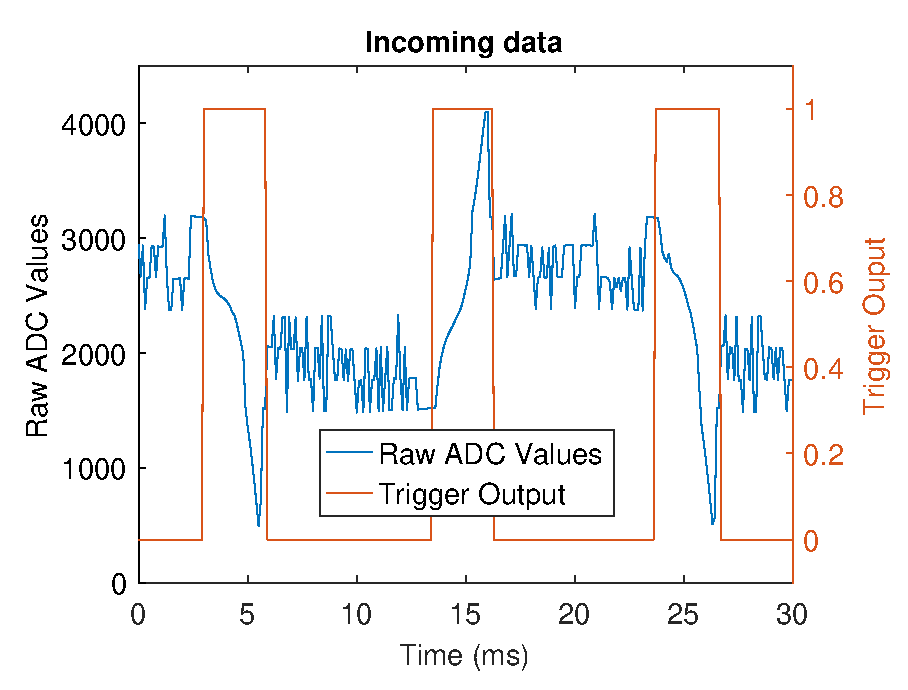
\includegraphics[width=0.7\textwidth]{chapters/evaluation-chapters/hardware/ac/raw-ac-testbed-adc-data.eps}
    \caption{Incoming data to the AC current sampler. The raw ADC values are plotted as well as the triggering circuit output.}
  \label{fig:raw-ac-testbed-adc-data-testbed}
\end{figure}

